\documentclass{beamer}
\usetheme{PaloAlto}
\usepackage{lmodern}
\author{Ravshanbek Khodzhimatov \\Thesis Advisor: Assoc. Prof. Dr. Tolga Umut Kuzuba\c{s}}
\title{Welfare Effects of Individualizing Life-Cycle Pension Investments to Households in Turkey}
\subtitle{Master's Thesis}
\usepackage{amsmath}
\usepackage{booktabs}
\usepackage{graphicx}
\usepackage{amsfonts}
\usepackage{geometry}
\usepackage{nameref}
\usepackage{tikz}
\beamertemplatenavigationsymbolsempty


%%%%%%%%%%%%%%%%%%%%%%%%%%%%%%%%%%
\begin{document}

\begin{frame}
\titlepage
\end{frame}

\section{Introduction}

\begin{frame}[allowframebreaks]{Introduction}
  \begin{itemize}
	\item Retirement is one of the most important investment decisions we face in our lives.
	\item Current investment menus are either too simplistic and inefficient or too complicated and unintuitive.
	\item Most individuals find active involvement in investment too complex.
	\item Lifecycle investments --- investments that solve for asset allocations separately for every age, as opposed to fixed investments.
	\item Naive investments --- asset allocations that do not consider indivdual characteristics. 

\framebreak

\begin{table}
	\centering
	\caption{Largest Turkish Pension Funds}
	\begin{tabular}[H]{lc}
		\hline
		Fund name&Fund size\\
		\hline
		Anadolu Hayat Emeklilik&8.7 bln\\
		Garanti Emeklilik ve Hayat&7.4 bln\\
		AvivaSA Emeklilik ve Hayat&9.1 bln\\
		Allianz Yasam ve Emeklilik&6.8 bln\\
		Vakif Emeklili&3.5 bln\\
		\hline
	\end{tabular}\\
	Source: Pension Monitoring Center (2016)
\end{table}
	
  \end{itemize}
\end{frame}


\section{Literature Review}

\begin{frame}[allowframebreaks]{Literature Review}
  \begin{itemize}
	\item Markowitz's Mean-Variance Analysis --- maximize return while minimizing volatility:
\begin{center}
  $\displaystyle\max_{\alpha} \{ E[R_p] - \frac{\gamma}{2}\sigma^2_p \}$
\end{center}
solution:
\begin{center}
	$\alpha = \frac{E[R] - R_f}{\gamma\sigma^2}$
\end{center}
where $\alpha$ is risky asset share in portfolio.

	\item Markowitz derived fixed solution and didn't capture lifecycle differences.

\framebreak

	\item Merton (1971) added human capital (discounted sum of future fixed wage) into the model:
  
\begin{center}
	$\alpha_t = \frac{\mu - R_f}{\gamma \sigma^2}\left(1+\frac{H_t}{W_t}\right)$
\end{center}

	\item $H_t/W_t$ changed over time and captured lifecycle effect. Moreover, since young people had higher human capital, they would be more aggressive than Markowitz, and old people would converge to Markowitz.

	\item Bodie et al. (1992) solved Merton for variable wage and used dynamic optimization to solve it. 
\framebreak
	
	\item Cocco et al. (2005) did similar analysis and added the following heuristic:


\begin{center}
	$\alpha_t = \begin{cases} 100\% & t<40\\(200-2.5t)\% & t\in[40,60]\\50\% & t>60 \end{cases}$,
\end{center}

	\item Flavin and Yamashita (2002) added housing capital as well and concluded that if individuals possessed housing, they would be even more aggressive. Solution was still done using dynamic optimization.

\framebreak

	\item Munk (2016) reinvented analytical solution to the problem.

\begin{center}
	$ \displaystyle\max_{\pi} \{ E[\frac{W_1}{W_0}] - \frac{\gamma}{2} var(\frac{W_1}{W_0}) \} $
\end{center}

where total wealth is a sum of financial and human wealth: $W_t = F_t + L_t$ and human capital has returns $r_L \sim (\mu_L, \sigma_L)$.

\begin{center}
	$\pi^* = \frac{1}{\gamma} \frac{W_0}{F_0} \cdot \Sigma^{-1} (\mu - r_f \cdot 1) - \frac{L_0}{F_0} \cdot \Sigma^{-1} cov(r,r_L)$
\end{center}


  \end{itemize}
\end{frame}

\section{Model}

\begin{frame}[allowframebreaks]{Model}
  \begin{itemize}
	\item We use Olear's (2016) approach to model labor income:

\begin{center}
	$Y_{i,t+1} = 
	\begin{cases}
		Y_{it} (1 + g_{i,t+1} + \xi_t + \omega_{it}), & t \leq T \\
		\lambda (1 + f(T, Z_{iT}) + v_{iT}), & t > T
	\end{cases}	
	$
\end{center}

	\item We model two risky assets and a wage as correlated discrete series:\\
$\frac{\Delta S_{t+1}}{S_t} = \mu_s + \sigma_s \cdot \epsilon_{st}$\\
$\frac{\Delta H_{t+1}}{H_t} = \mu_h + \sigma_h \cdot \left(\rho_{hs}\epsilon_{st} + (\sqrt{1-\rho^2_{hs}})\epsilon_{ht}\right)$\\
$\frac{\Delta Y_{t+1}}{Y_t} = \mu_v + \sigma_v \cdot \left(\rho_{ys}\epsilon_{st} + \left(\frac{\rho_{yh} - \rho_{sh}\rho_{sy}}{\sqrt{1-\rho^2_{sh}}}\right)\epsilon_{ht} + \left(\sqrt{1-\rho^2_{ys}-(\frac{\rho_{yh} - \rho_{sh}\rho_{sy}}{\sqrt{1-\rho^2_{sh}}})^2}\right)\epsilon_{vt}\right)$

\framebreak

	\item Welfare measurement --- we use CRRA utility:

\begin{center}
	$E_1[U(c)] = E_1 \left[\displaystyle\sum^T_{t=1} \delta^{t-1} \displaystyle\prod^{t-1}_{j=0} p_j \cdot \frac{c^{1-\gamma}_{it}}{1-\gamma}\right]$
\end{center}

where $p_k$ is the probability of survival from time $k-1$ to time $k$.

	\item We omitted the bequest motives from the original formulation, thus retired person consumes all of his income at any given time.

\framebreak

	\item We used Munk's solution without housing:

\begin{center}
	$\pi_{t+1} = \frac{\mu_s - r_f}{\gamma \sigma^2_s}  + \frac{L_t}{F_t} \cdot \left(\frac{\mu_s - r_f}{\gamma \sigma^2_s} - \frac{\rho_{SL}\sigma_L}{\sigma_S} \right)$
\end{center}

	and with housing:

\begin{center}
	$\pi_{t+1} = \frac{1}{\gamma (1 - \rho^2_{SH}) \sigma_S} \cdot \frac{W_t}{F_t} \left( \frac{\mu_s - r_f}{\sigma_S} - \rho_{SH} \frac{\mu_h - r_f}{\sigma_h} \right) - \frac{L_t}{F_t} \cdot \frac{\sigma_L}{\sigma_S} \frac{\rho_{SL} - \rho_{SH}\rho_{HL}}{1 - \rho^2_{SH}}$
\end{center}
\begin{center}
	$\pi_{h,t+1} = \frac{1}{\gamma (1 - \rho^2_{SH}) \sigma_H} \cdot \frac{W_t}{F_t} \left( \frac{\mu_h - r_f}{\sigma_h} - \rho_{SH} \frac{\mu_s - r_f}{\sigma_s} \right) - \frac{L_t}{F_t} \cdot \frac{\sigma_L}{\sigma_h} \frac{\rho_{HL} - \rho_{SH}\rho_{SL}}{1 - \rho^2_{SH}}$
\end{center}
\begin{center}
	$\pi_{R_f} = \left( 1 - \pi - \pi_h \right)$
\end{center}

\framebreak
	
	\item Retirement income --- accumulated financial wealth is repaid back in annuities.
	\item Reverse mortgages --- housing wealth is reinvested for annuities in return of inheriting a house to the payer (no bequest motives) 

\begin{center}
	$W_{57} = H_{57} + MP$
\end{center}

	\item Annuity is equal to:
$\frac{W_{57}}{1+\sum^{100}_{t=58} \frac{p_t}{1+r_f}}$ 
	
	\item Welfare calculation --- we convert annuity stream into consumption (considering the inflation) and plug into CRRA expected utility function.

  \end{itemize}
\end{frame}

\section{Data Structure and Sources}

\begin{frame}[allowframebreaks]{Data Structure and Sources}
  \begin{itemize}

	\item Stock rates of return are obtained from Borsa Istanbul BIST30 index:

\begin{figure}
	\centering
	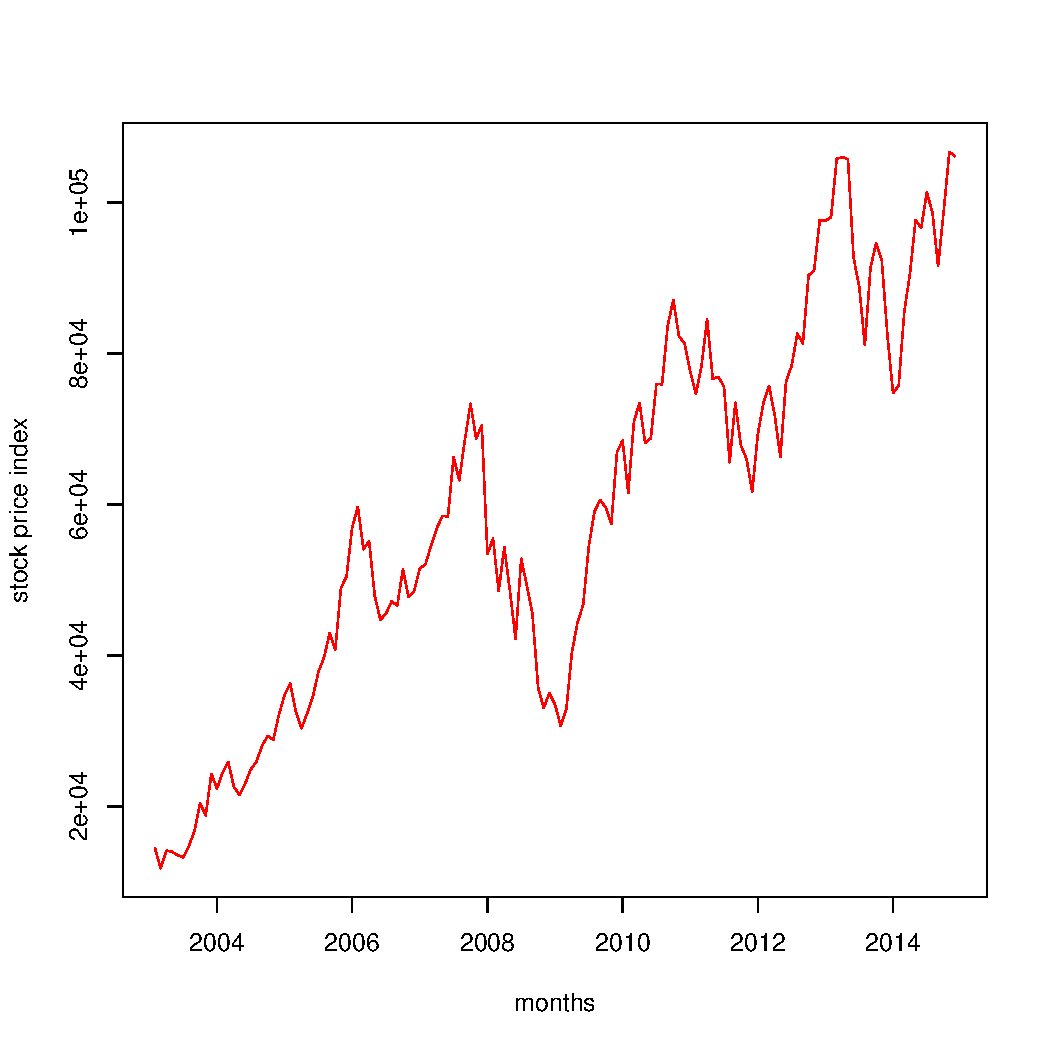
\includegraphics[scale=0.25]{figs/bist.pdf}
	\caption{BIST30 Turkish stock market performance index}
\end{figure}

\framebreak


	\item Housing returns are obtained from Reidin AEINDEXF index:

\begin{figure}
	\centering
		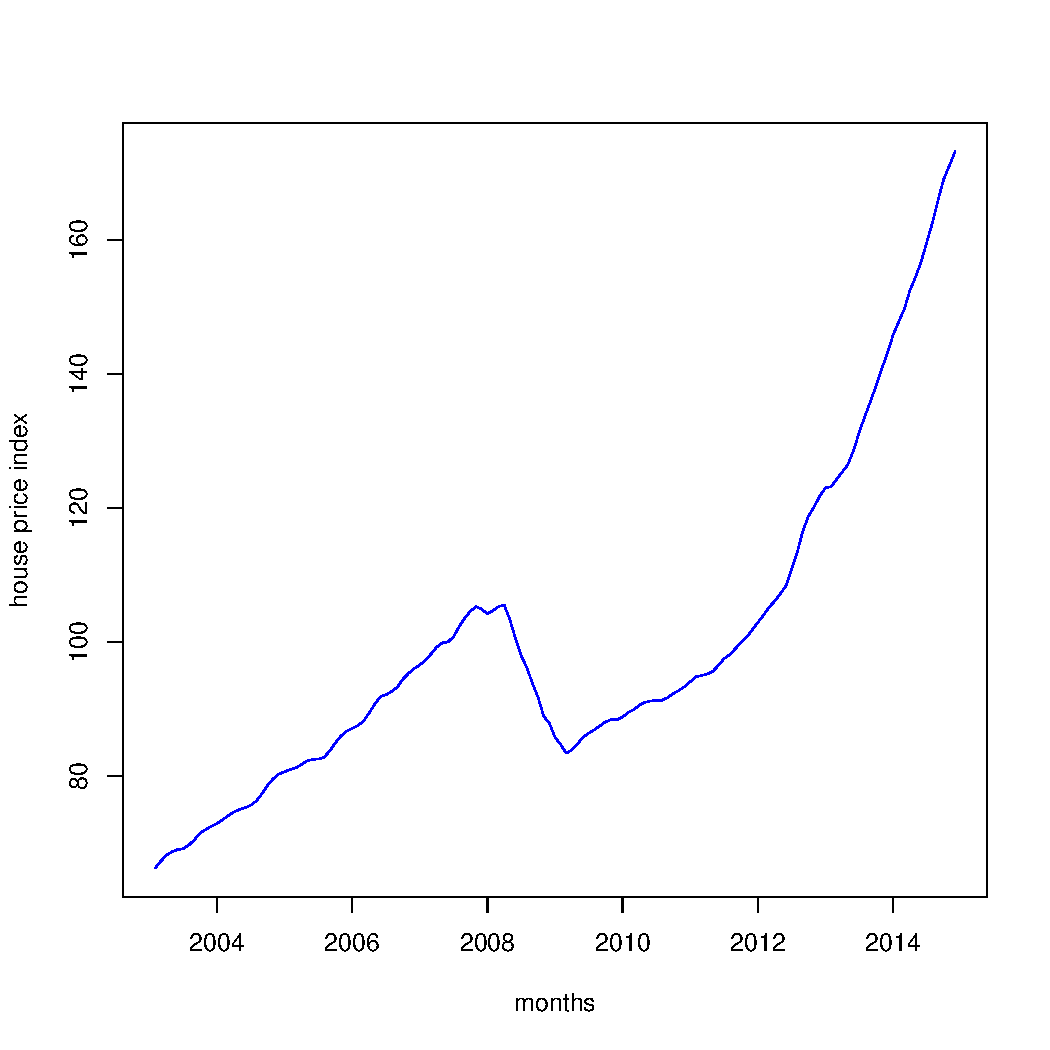
\includegraphics[scale=0.25]{figs/reidin.pdf}
		\caption{Reidin Turkish house price index}
\end{figure}

\framebreak

	\item Wage dynamics are obtained from TUIK Houshold Budget Survey (HBS) and Aktug, Kuzubas, Torul (2017) (notice the hump shape):

\begin{figure}[h]
	\centering
	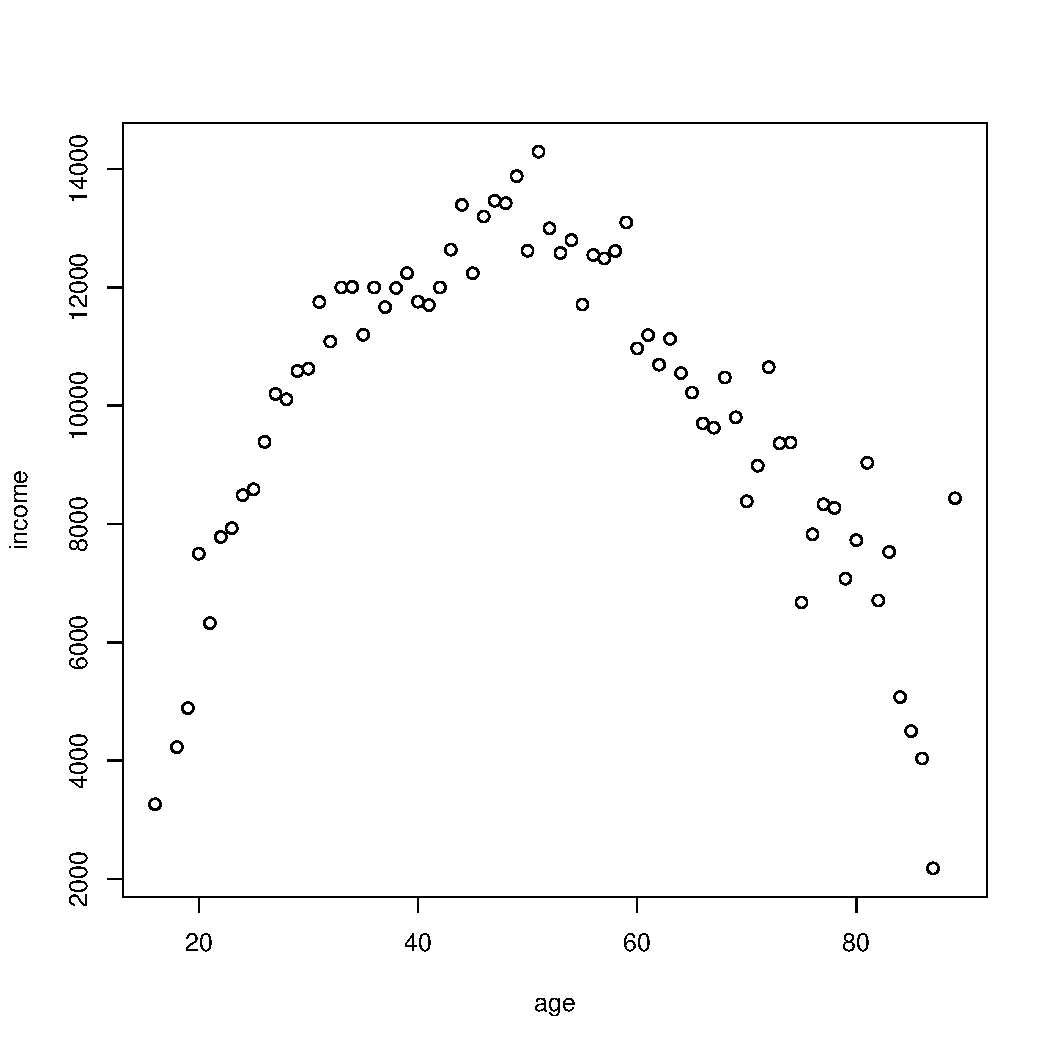
\includegraphics[scale=0.25]{figs/wage2median.pdf}
	\caption{Median Turkish salaries by age}
\end{figure}

\framebreak

	\item We start with 28 years old individual, who invests for 30 years until retirement at 57.
	\item In line with Torul et al. (2018), $\delta = 0.89$
	\item Stock returns: $23.2\%$ with standard deviation $36\%$
	\item Bond returns obtained from OECD Data Bank (2018) and are equal to $10.8\%$
	\item Housing capital appreciation: $11.3\%$ with standard deviation $5.2\%$

\framebreak

\begin{table}
	\centering
	\caption{Benchmark Parameters}
	\begin{tabular}[c]{lll}
		\hline
		Parameter&Description&Value\\
		\hline
		$Y$&Beginning age&$28$\\
		$R$&Retirement age&$57$\\
		$T$&Lifespan (years)&$100$\\
		$\gamma$&Risk aversion&$5$\\
		$\beta$&Discount rate&$0.89$\\
		$r_f$&Risk-free rate&$0.108$\\
		$\pi$&Average inflation rate&$0.084$\\
		\hline
		$\mu_s$&Expected stock returns&$0.232$\\
		$\mu_h$&Expected housing returns&$0.113$\\
		$\sigma_s$&Stock returns volatility&$0.36$\\
		$\sigma_h$&Housing returns volatility&$0.052$\\
		$\sigma_w$&Wage growth volatility&$0.056$\\
		$\rho_{hs}$&Housing-stock correlation&$0.24$\\
		$\rho_{hw}$&Housing-wage correlation&$0.37$\\
		\hline
	\end{tabular}
\end{table}

\framebreak 
	\item The data on survival probability for all ages is obtained from TUIK database

\begin{figure}[h]
	\centering
	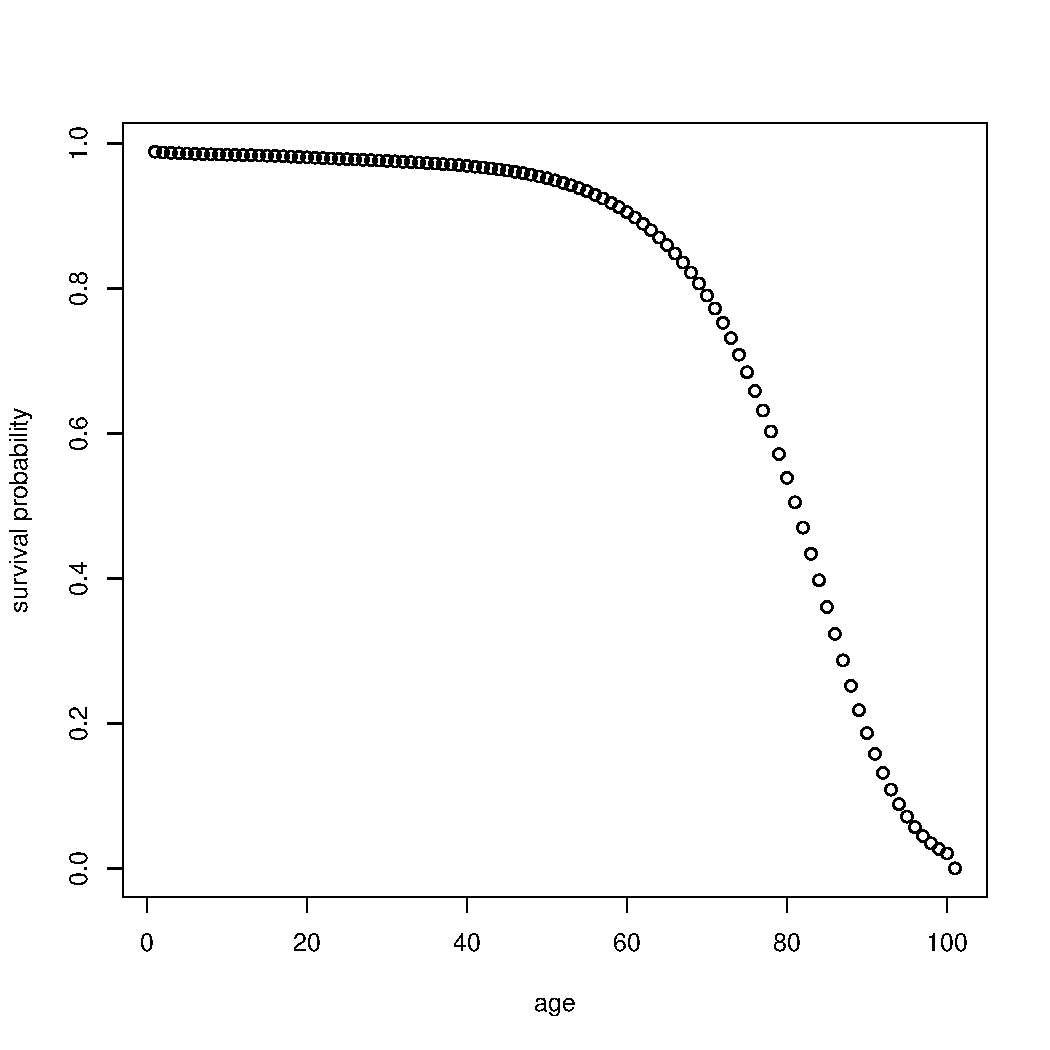
\includegraphics[scale=0.25]{figs/survival.pdf}
	\caption{Survival probabilities by age}
\end{figure}


\framebreak 

	\item We consider heterogeneity of agents as follows:
	\item Heterogeneity in education --- defined as difference in wage curve steepness

\begin{figure}[h]
	\centering
	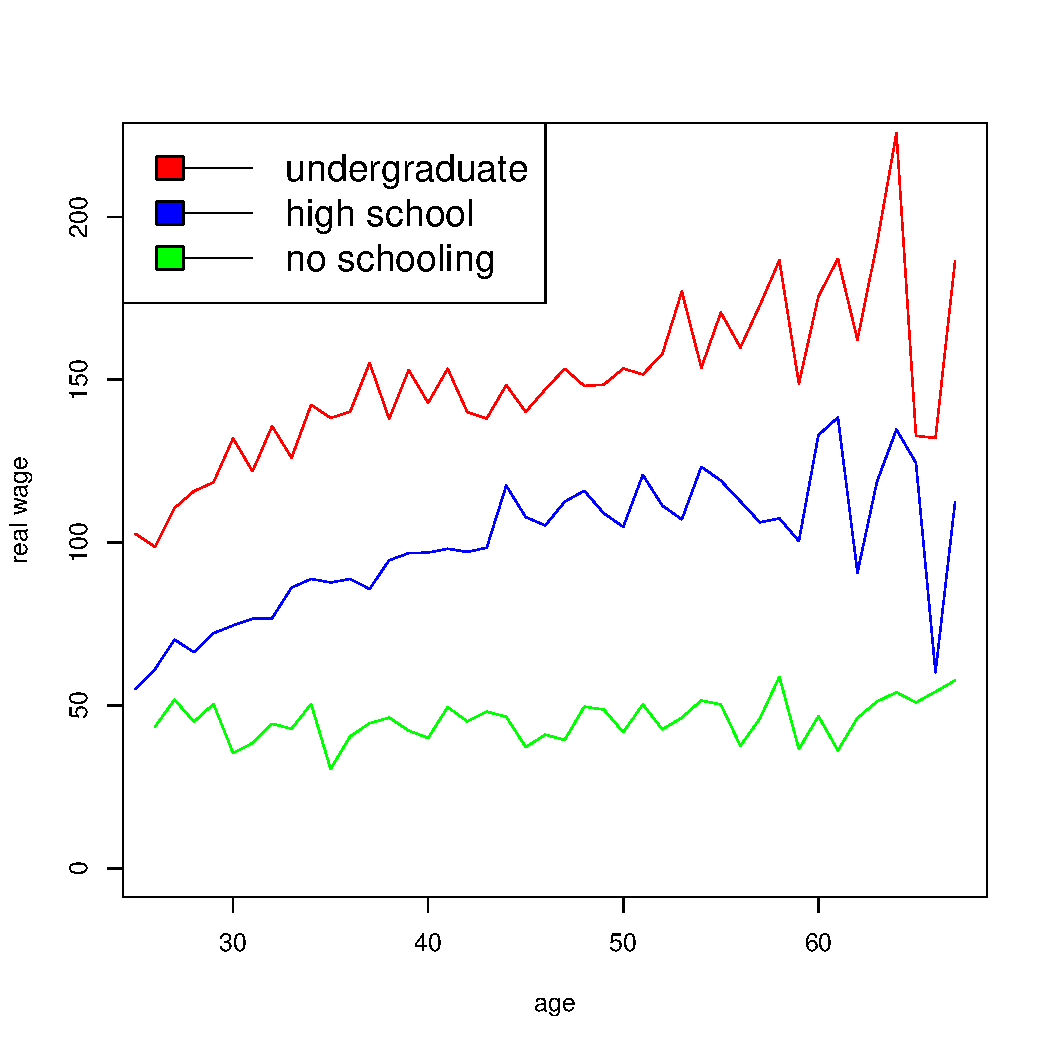
\includegraphics[scale=0.25]{figs/wage2educ.pdf}
	\caption{Lifetime wage dynamics by education level}
\end{figure}


\framebreak

	\item Performing kinked regressions results in the following three wage growth rates:

\begin{table}
	\centering
	\caption{Estimated Benchmark Wage Growth Rates $\mu_w$}
	\begin{tabular}[c]{l|ccc}
		Age&Flat&Moderate&Steep\\
		\hline
		0-35&0\%&3.5\%&6.5\%\\
		36-45&0\%&3\%&2\%\\
		46-60&0\%&0\%&0\%\\
	\end{tabular}
\end{table}

\framebreak

	\item Parameterized and actual wage curves

\begin{figure}[h]
		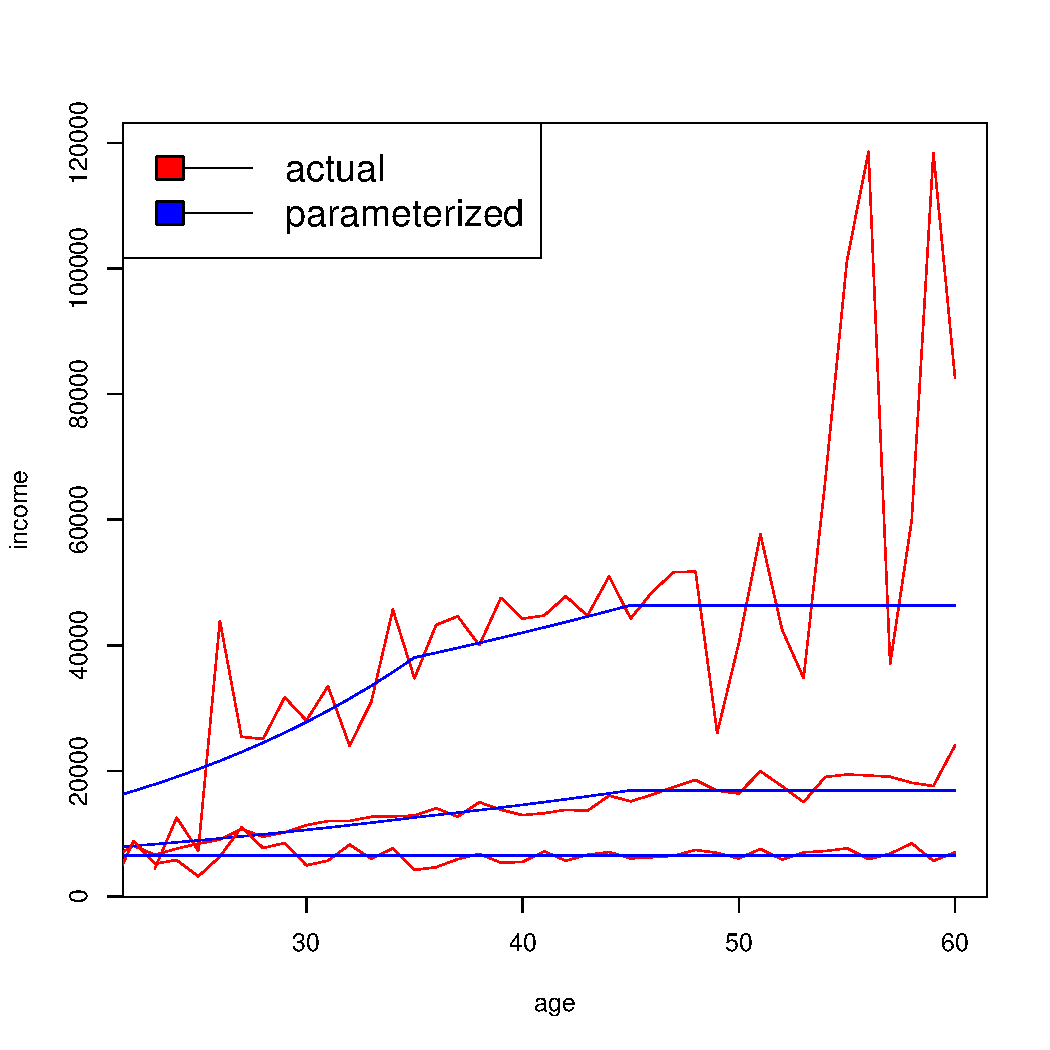
\includegraphics[scale=0.25]{figs/heterwage.pdf}
		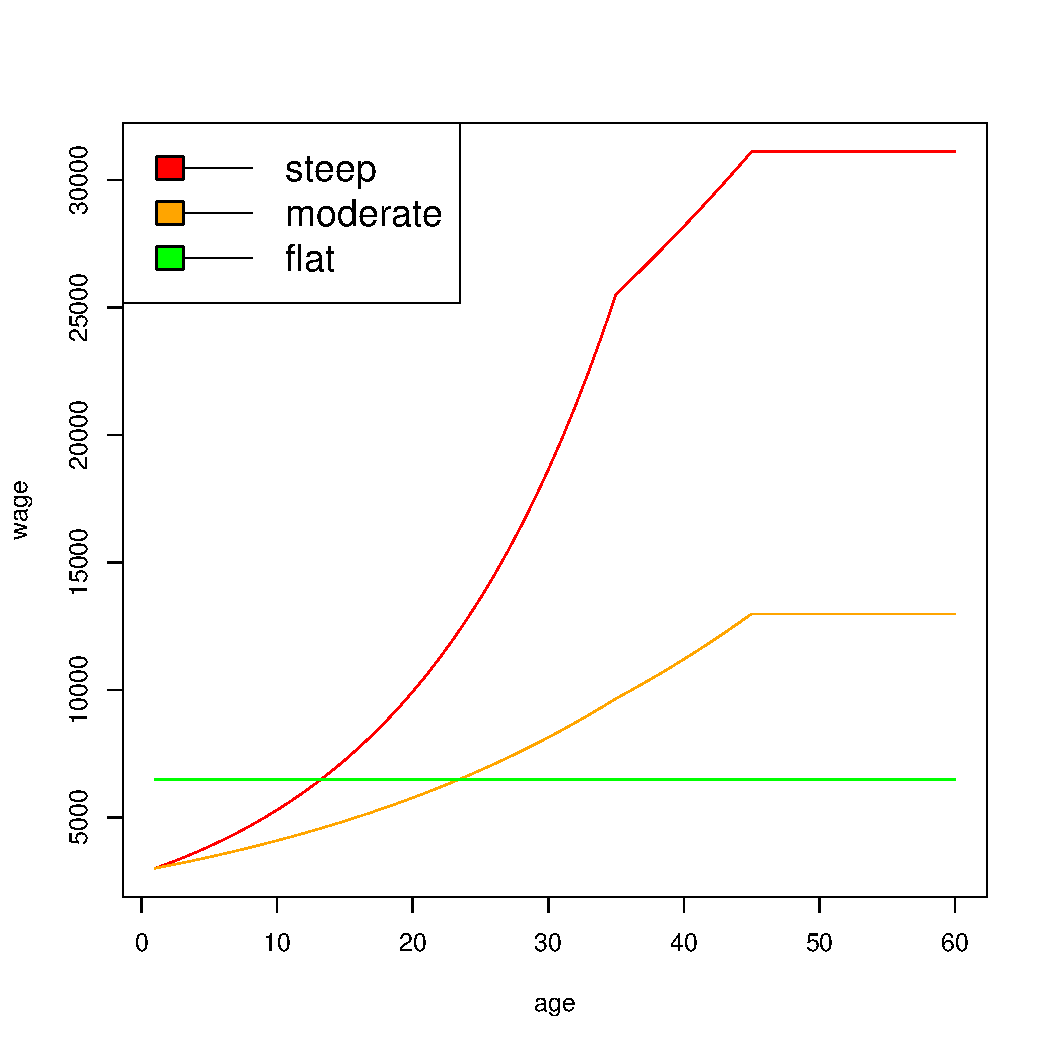
\includegraphics[scale=0.25]{figs/heterwageless.pdf}
\end{figure}


	\framebreak

	\item The investments are done from $0.03\%$ of every wage from 28 to 56 years.
	\item Heterogeneity in sectors of work --- it is captured by differing stock-wage correlations
	\item Zero for agricultural sector / teaching
	\item As high as $0.4$ for financial sector
	\item $0.2$ in the middle
	\item Notice movements during 2008 crisis

\begin{figure}[h]
	\centering
	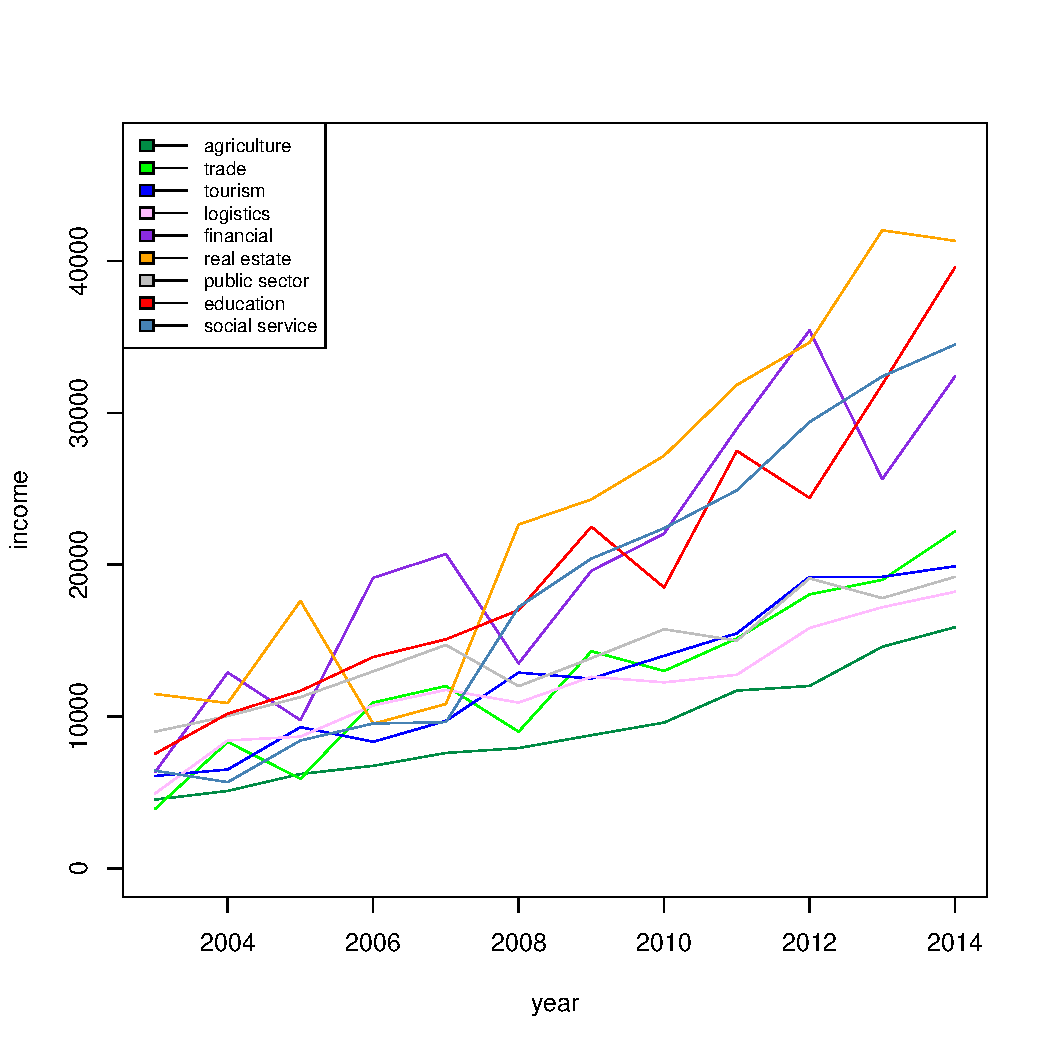
\includegraphics[scale=0.3]{figs/wage2sec.pdf}
	\caption{Historical wage dynamics by sector}
\end{figure}

\framebreak

	\item Individual heterogeneity --- it is captured by different risk aversion levels:

\begin{table}
	\centering
	\caption{Coefficients of Risk Averion}
	\begin{tabular}[c]{r|cccc}
		Values&Torul&low&default&high\\
		\hline
		$\gamma$&1.5&3&5&10\\
	\end{tabular}
\end{table}
	
\framebreak

	\item We constructed human capital and financial capital series taking the heterogeneities into consideration:
	\item $H_t/F_t$ is declining in $t$ --- optimal risky asset share is declining

\begin{figure}[h]
		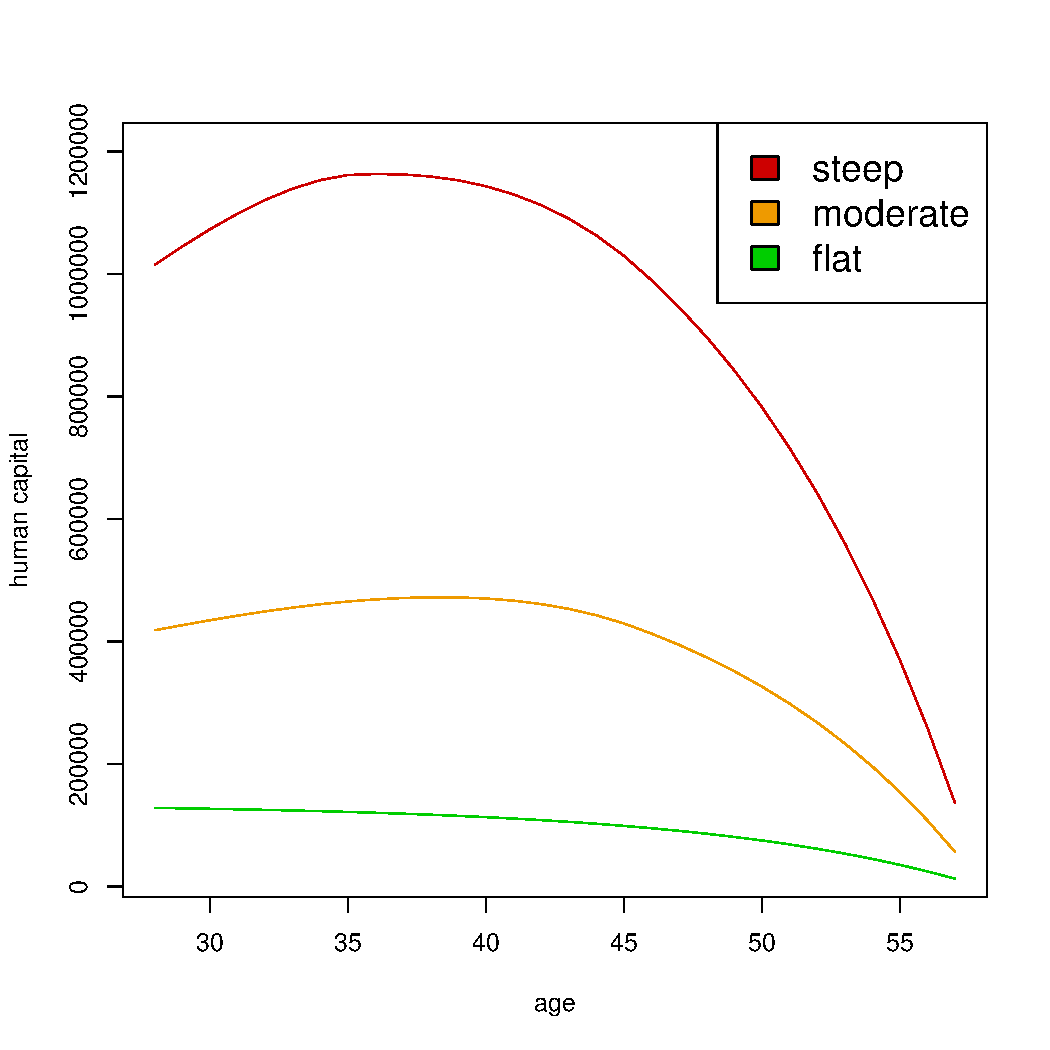
\includegraphics[scale=0.25]{figs/humancapital.pdf}
		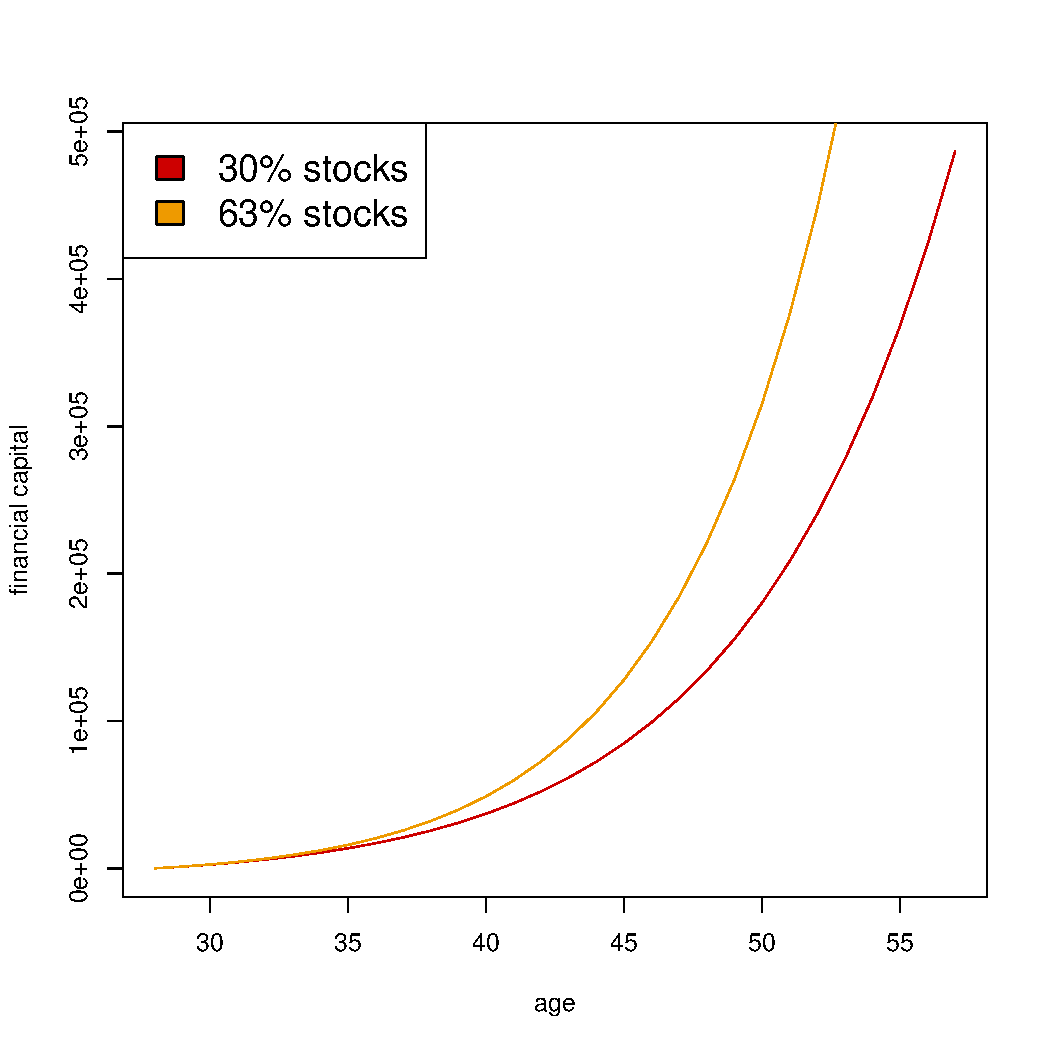
\includegraphics[scale=0.25]{figs/fincapital.pdf}
\end{figure}

  \end{itemize}
\end{frame}

\section{Results}

\begin{frame}[allowframebreaks]{Results}
  \begin{itemize}
	\item First, we list default and derived investment strategies
	\item Then we calculate the capital movements using these strategies
	\item We obtain total wealth before retirement and annuitize it
	\item We convert annuities into consumption levels considering inflation
	\item We plug consumption levels into expected utilities
	\item We compare resulting utilities and conclude

\framebreak

	\item Default strategies

\begin{figure}[h]
	\centering
	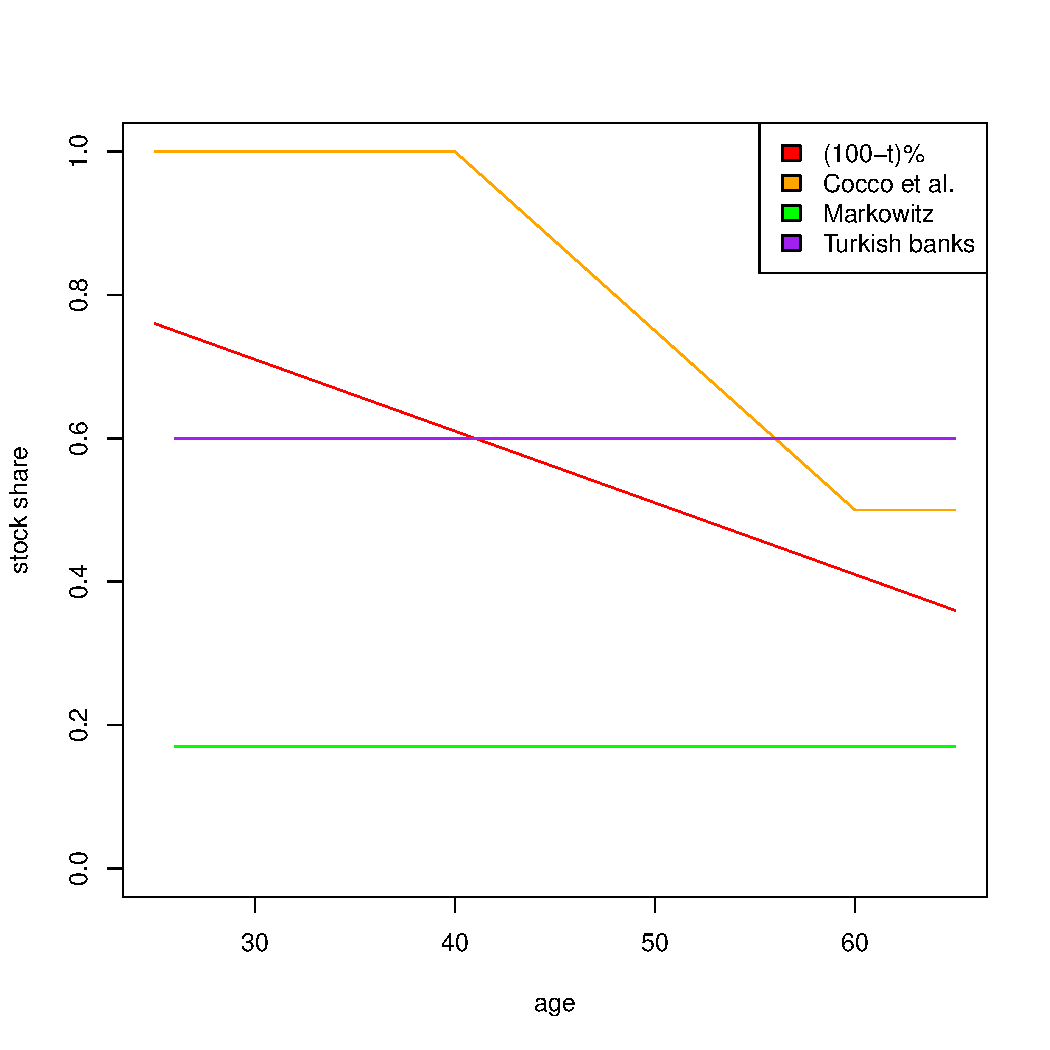
\includegraphics[scale=0.25]{figs/defaults.pdf}
	\caption{Default portfolio allocations of stock investments}
\end{figure}
		

\framebreak


	\item Several individualized solutions ($\gamma=1.5,3,5,10$):

\begin{figure}
		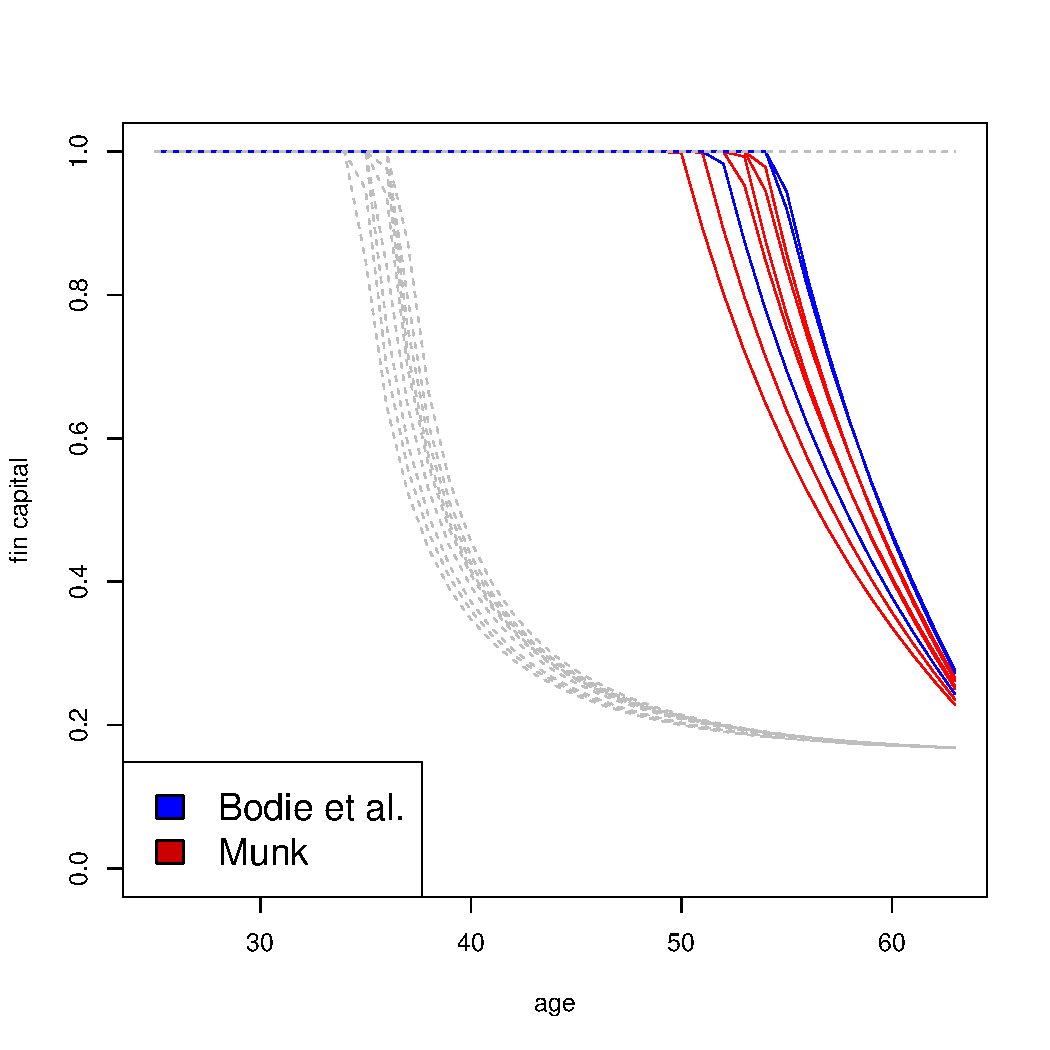
\includegraphics[scale=0.25]{figs/individuals15.pdf}
		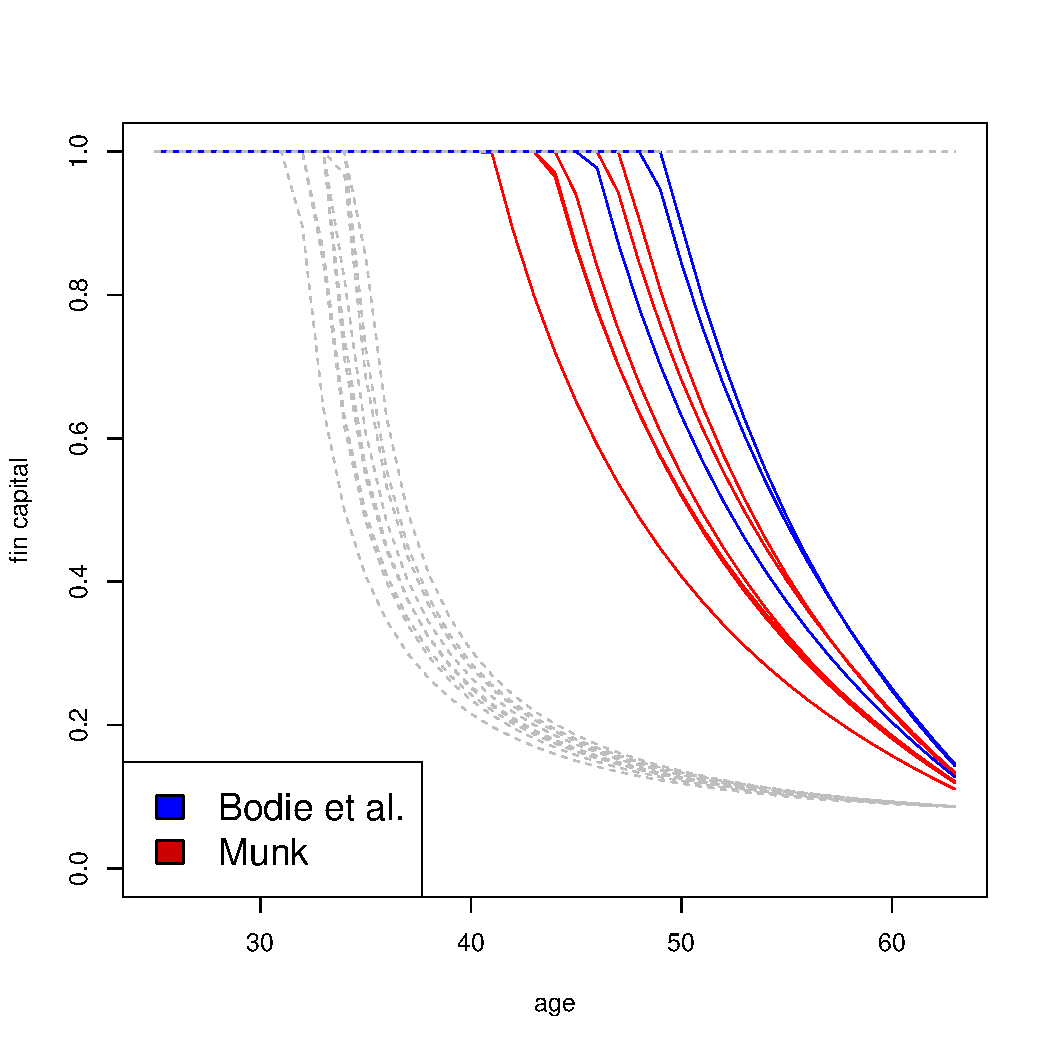
\includegraphics[scale=0.25]{figs/individuals3.pdf}
		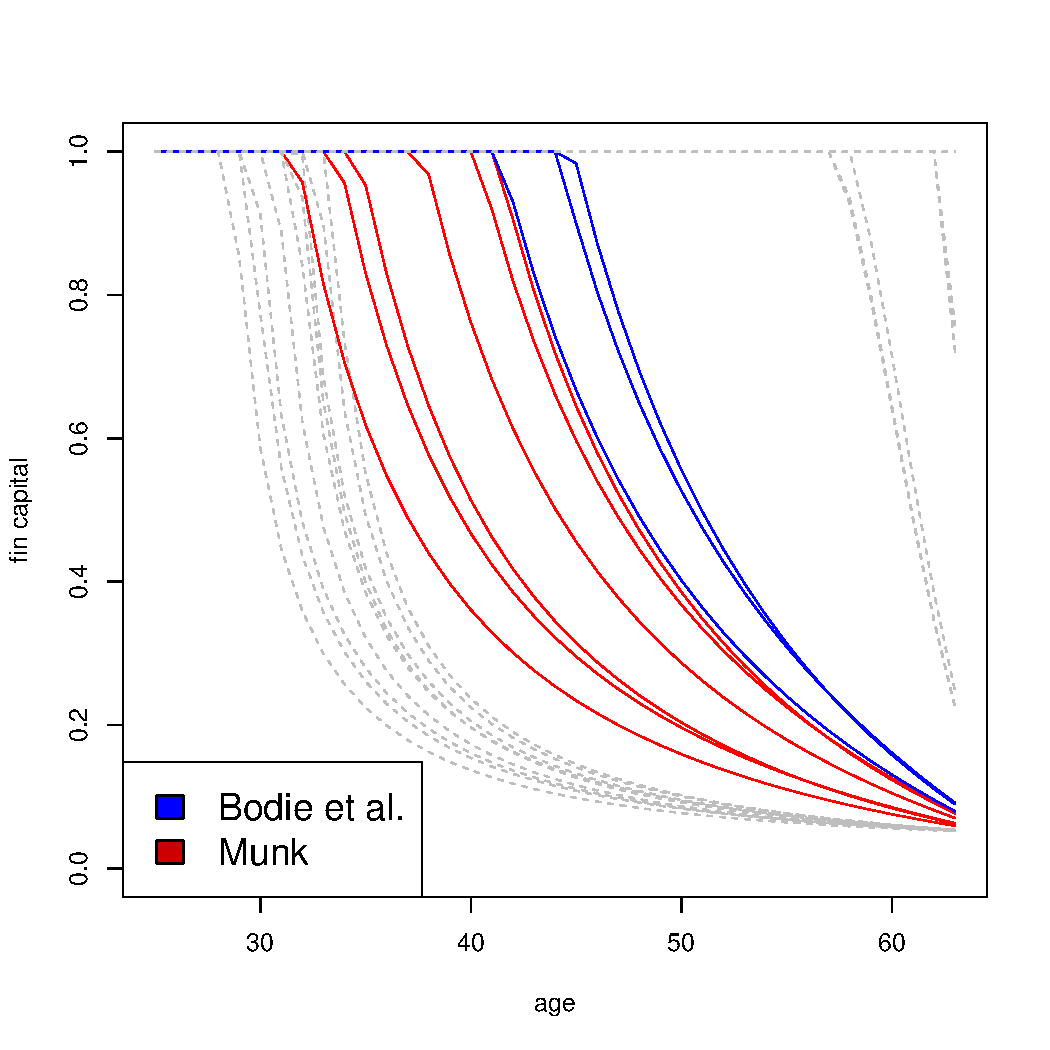
\includegraphics[scale=0.25]{figs/individuals5.pdf}
		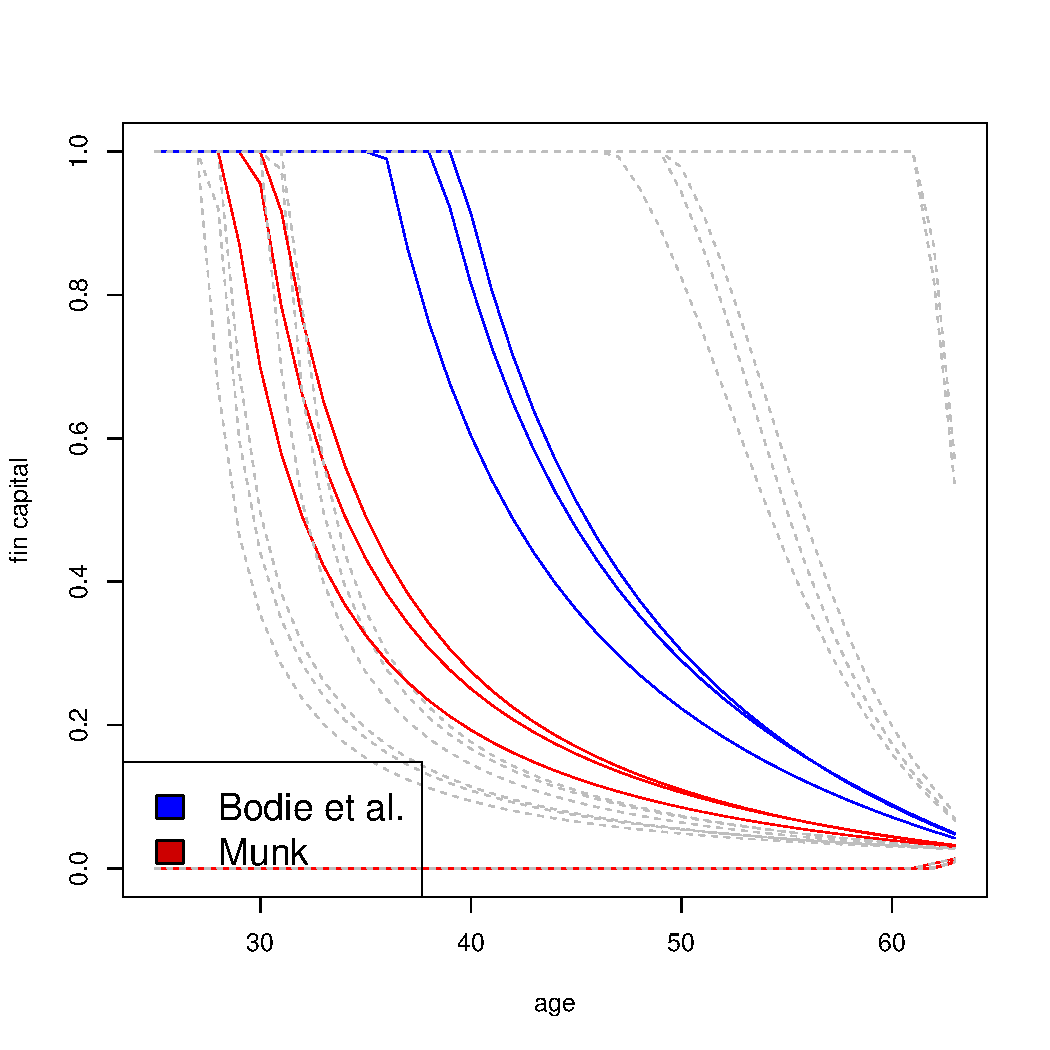
\includegraphics[scale=0.25]{figs/individuals10.pdf}
\end{figure}

\framebreak

	\item Note that for small stock-wage correlations, Munk's solution without housing is equivalent to Merton's solution
	\item Note that for smaller risk aversion, households invest more aggressively
	\item Note that flat wagers are less aggressive than steeper wagers
	\item Munk's solution with housing are presented below.
	\item Left graph is optimal stock share and right graph is optimal housing share
	\item Graphs are done for $\gamma=1.5,3,5,10$
\framebreak

\begin{figure}[H]
		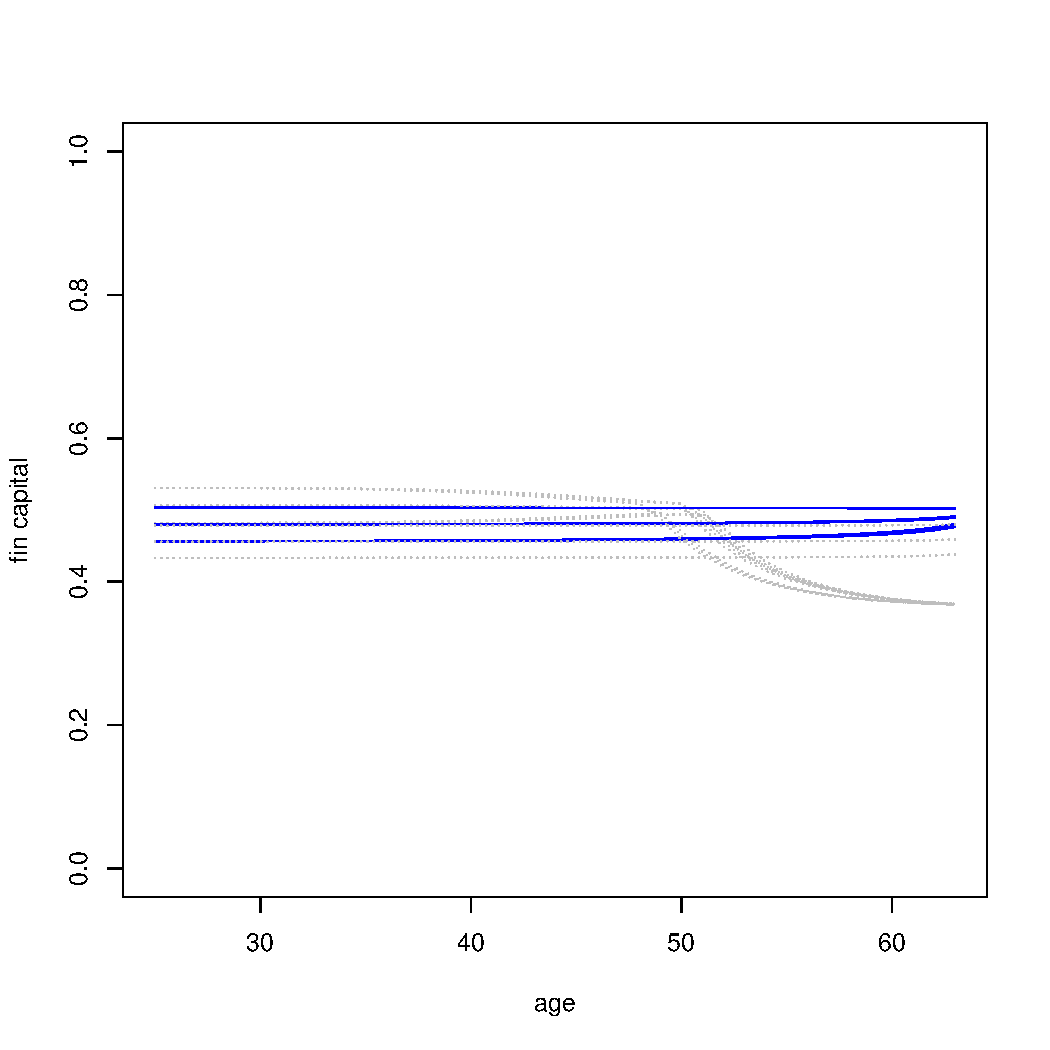
\includegraphics[scale=0.25]{figs/smunkhouse15.pdf}
		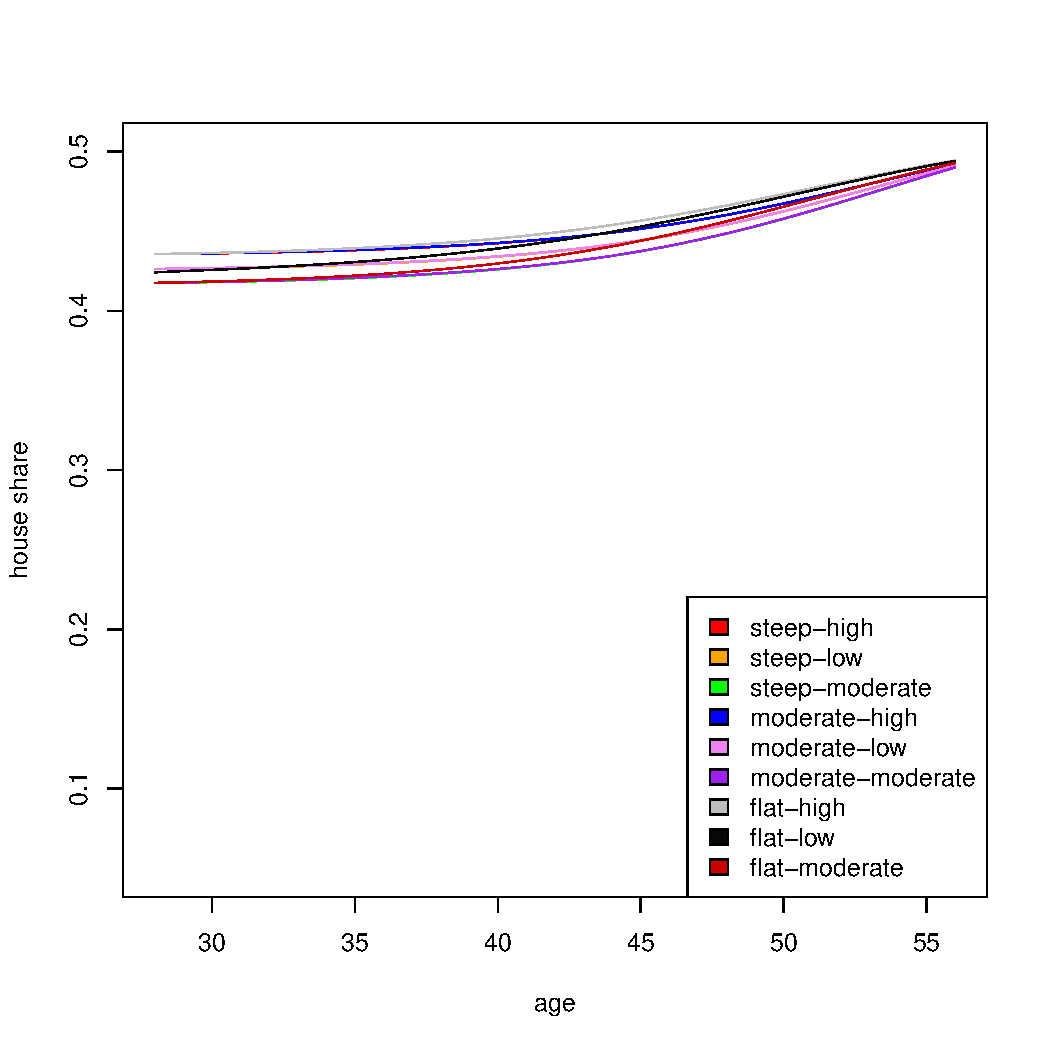
\includegraphics[scale=0.25]{figs/hmunkhouse15.pdf}
		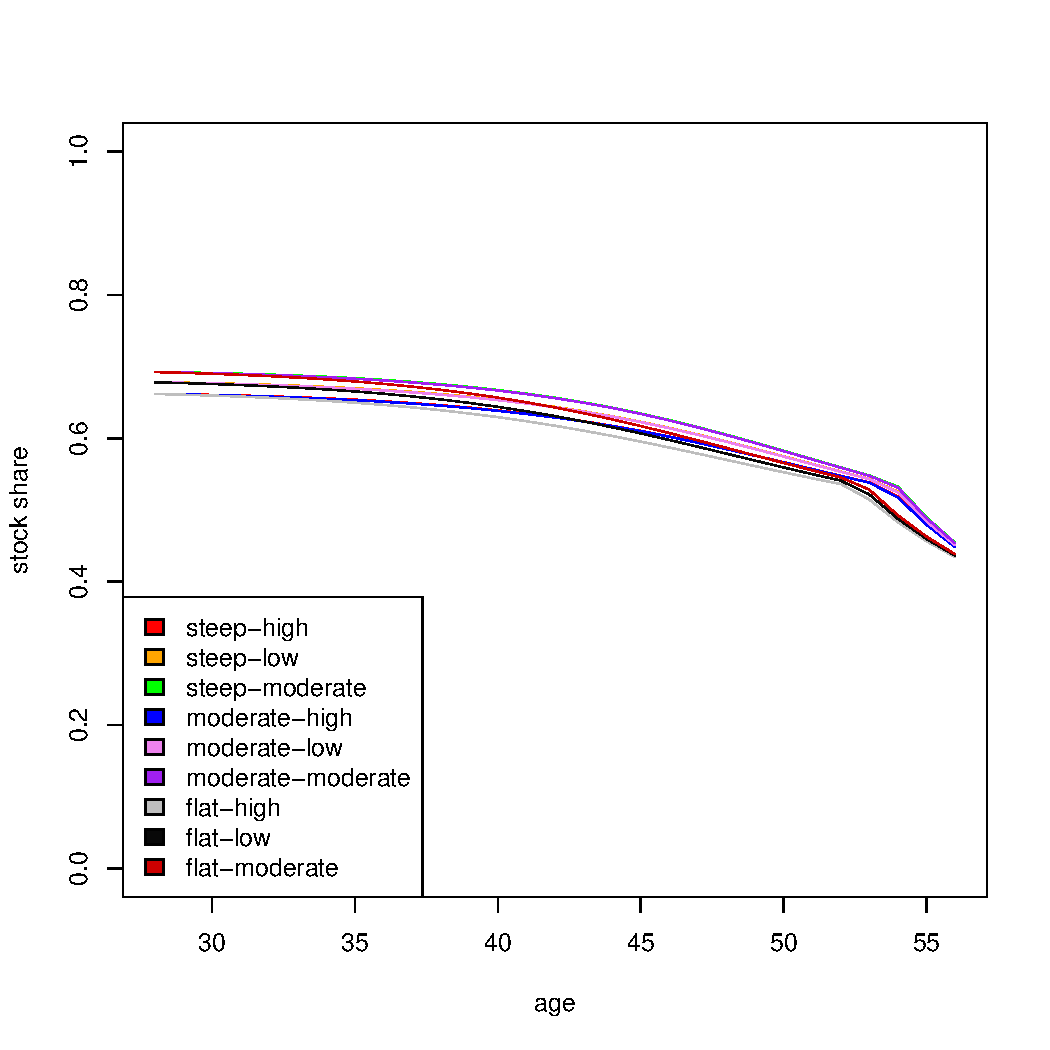
\includegraphics[scale=0.25]{figs/smunkhouse3.pdf}
		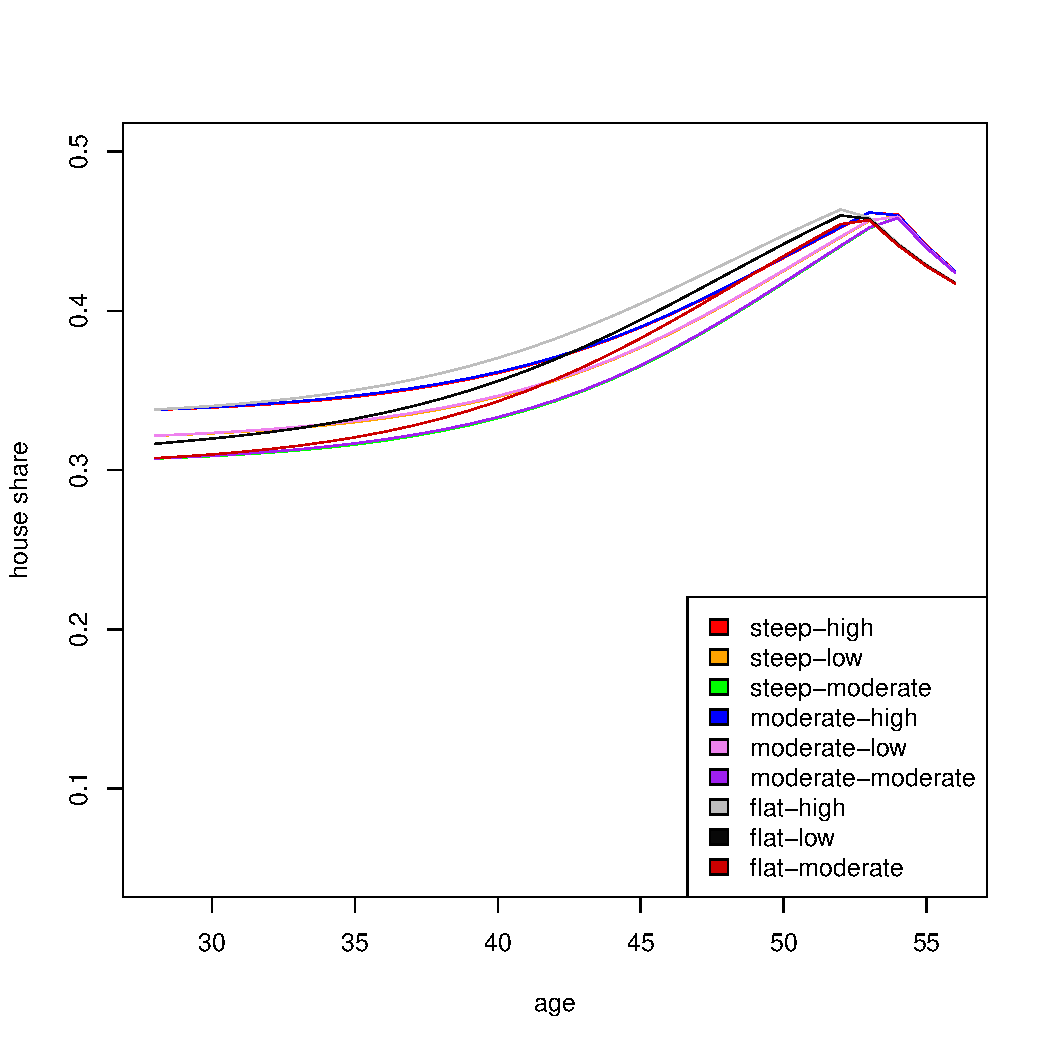
\includegraphics[scale=0.25]{figs/hmunkhouse3.pdf}
		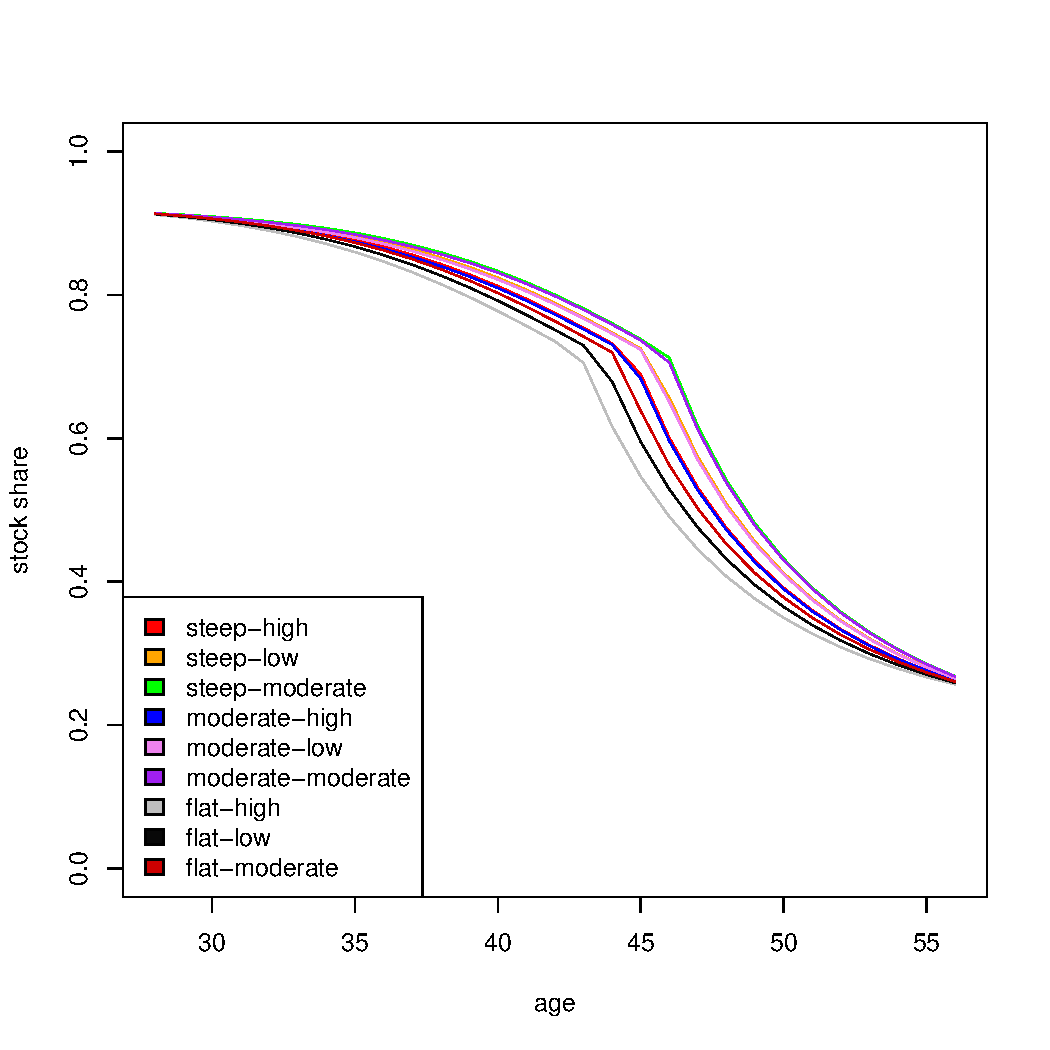
\includegraphics[scale=0.25]{figs/smunkhouse5.pdf}
		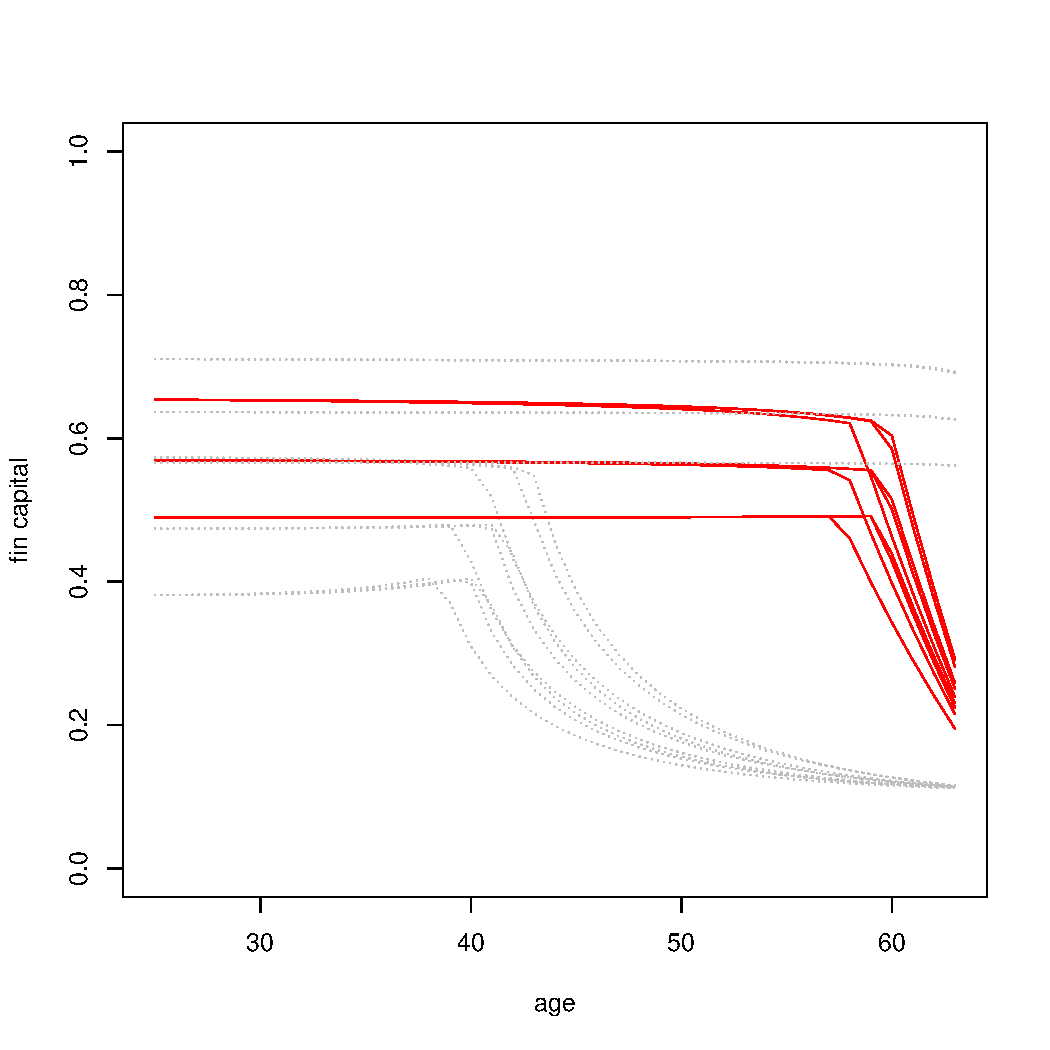
\includegraphics[scale=0.25]{figs/hmunkhouse5.pdf}
		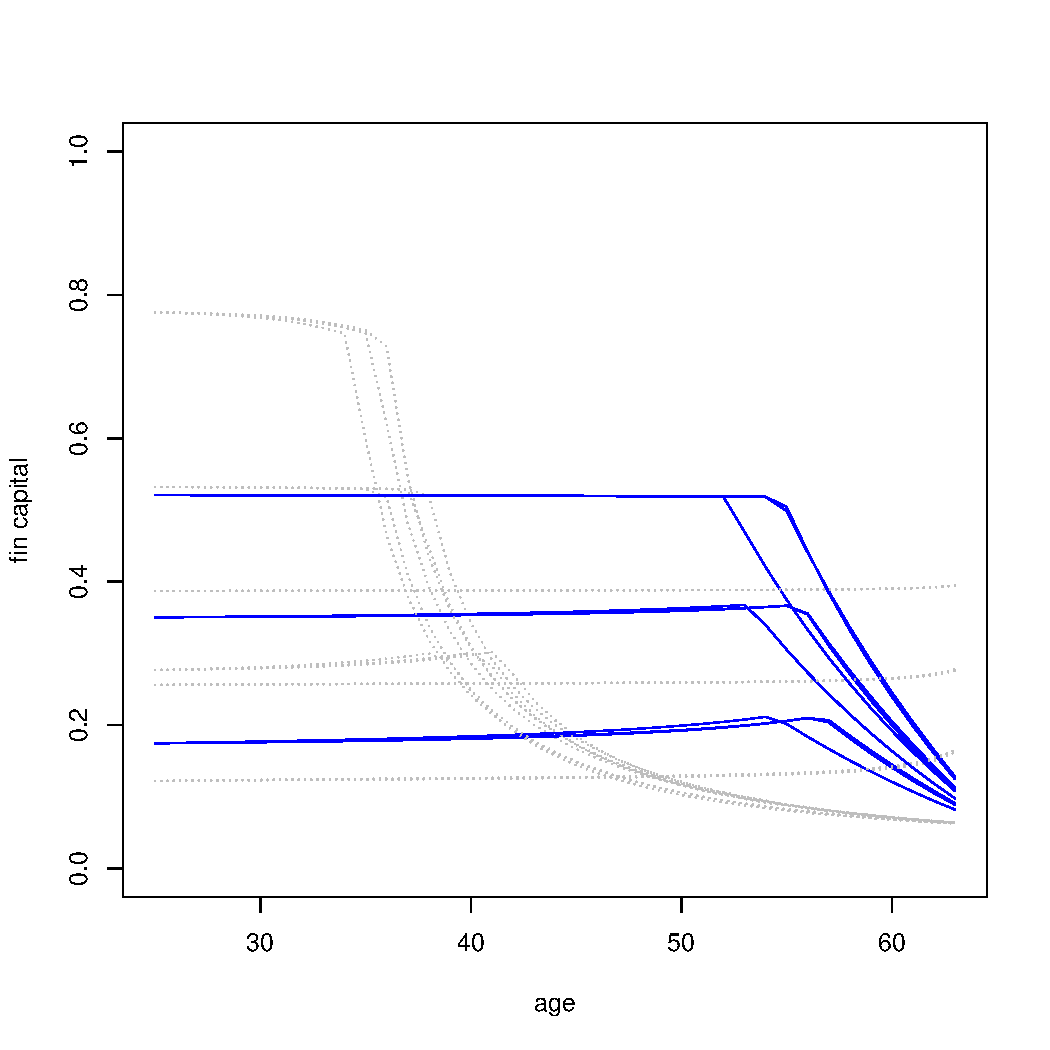
\includegraphics[scale=0.25]{figs/smunkhouse10.pdf}
		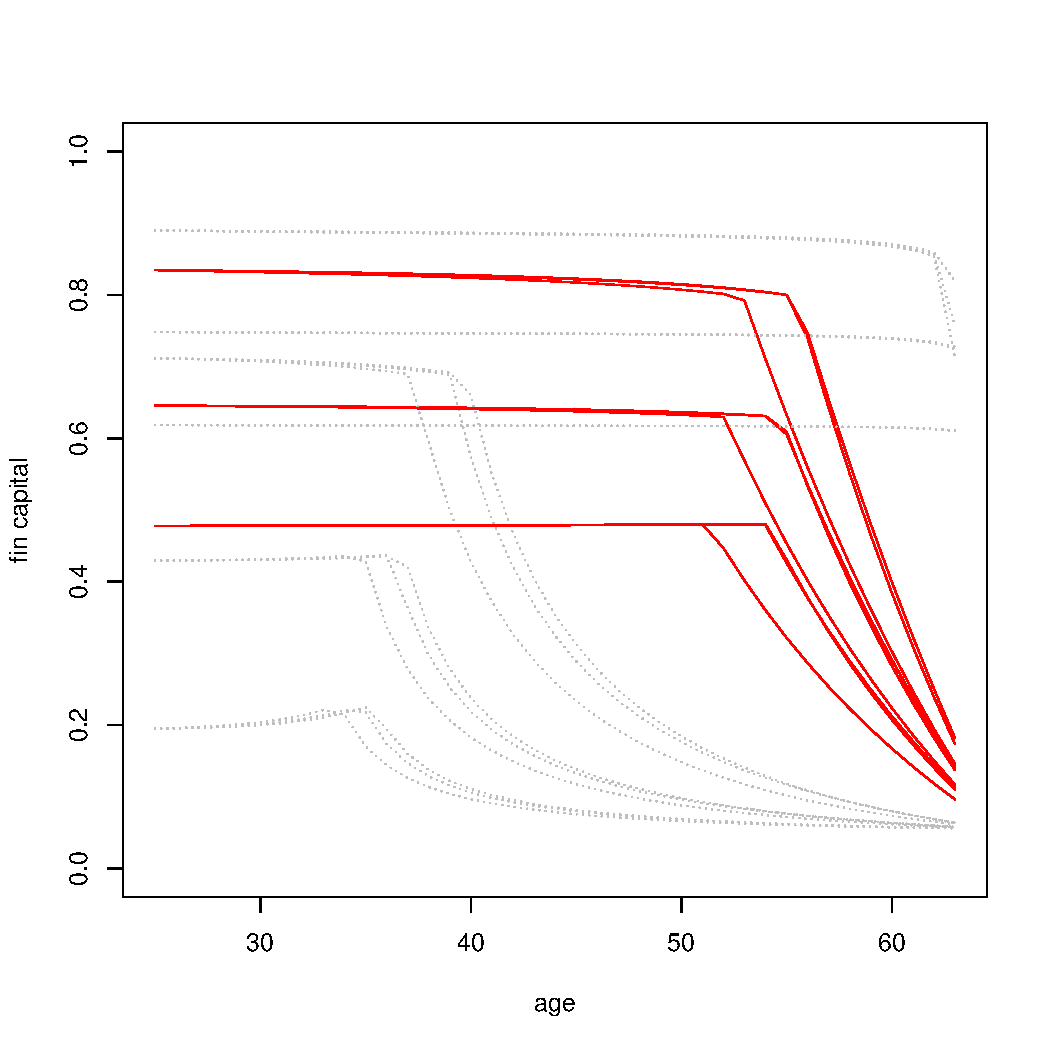
\includegraphics[scale=0.25]{figs/hmunkhouse10.pdf}
\end{figure}


\framebreak

	\item In line with Munk, the stock-house allocation is done as follows:
		\begin{itemize}
			\item If optimal stock and housing allocations sum up to a number greater than $1$, then we allocate our wealth proportionately between the two
			\item If optimal stock and housing allocations sum up to a number less than $1$, then we allocate those very shares and invest the rest into risk-free bonds 
		\end{itemize}
	\item The detailed tables with results are presented in Appendix E of our thesis

	\item Note that around age of 45 this sum falls below $1$ and kink happens. Bond share becomes nonnegative.
	\item Note that as risk aversion coefficeint increases, the kink happens earlier
	\item Note that for $\gamma=10$ the optimal housing is mostly negative and the sum is less than $1$, causing more allocation into risk-free bonds.
	\item Note that the steeper the wage curve is, the more aggressive the individual is
	\item Note that stock-wage correlation does not influence steep and flat wagers much
			

\framebreak

	\item After a lifetime of investing, the household accumulated various levels of wealth, summarized in the Table 5.1 of our thesis
	\item Looking at these total wealth levels, we can make early conclusions even before calculating utilities:
	\begin{itemize}
		\item Considering lifecycles, even naively, like $(100-age)\%$, is better than investing a fixed amount throughout lifetime
		\item Different stock-wage correlations don't make much difference in the outcome without housing, and make considerable difference in models with housing
		\item Stock-wage correlations are negatively correlated with total wealth
		\item The risk aversion is negatively correlated with total wealth for models without housing and positively --- for models with housing
		\item Default options are better for people with flat wage growth rate and worse for people with moderate or steep wage curves
	\end{itemize}

\framebreak

	\item Annuitization --- is done using the formula mentioned earlier,
	\item Consumption levels --- are calculated as amounts of consumption baskets that cost exactly $1$ $CPI_{r}$, which is equal to $100 TL$ at age 58.
	\item Consumption baskets increase in price every year by an inflation level $\pi = 8.4\%$
	\item Expected Utilities --- are calculated by plugging in survival probabilities, discount rate and corresponding risk aversion defined earlier and consumption levels just defined.
	\item Expected utilities are summarized in Table 5.3 of our thesis.

  \end{itemize}
\end{frame}

\section{Conclusion}

\begin{frame}[allowframebreaks]{Conclusion}
  \begin{itemize}

\item Naive lifecycle investment portfolios, such as $(100-age)\%$ don't overperform fixed-ratio Markowitz, because they don't take the risk aversion into consideration.
\item Cocco et al.'s $(200-2.5\cdot age)\%$ approximation is the best default portfolio. It is easy to interpret and captures lifecycle effect.
\item All models perform better for higher risk aversion and worse for lower risk aversion.
\item Higher stock-wage correlation considerably decreases the utility for moderate and flat wages, and doesn't affect much for steep wages.
\item Merton's solution outperforms Munk's solution without housing for low levels of risk aversion, and performs save for high level of risk aversion ($\gamma=10$).
\item Munk's solution with housing outperforms every other solution for high levels of risk aversion ($\gamma=10$).
\item Munk's solution with housing outperforms Munk's solution without housing for $\gamma=5,10$.
\item Markowitz's solution outperforms both Merton's and Munk's solutions for flat wages.
\item Individualizing lifecycles by wage growth rate and stock-wage correlation increases welfare for steep wagers and decreases welfare for flat wagers.
  \end{itemize}
\end{frame}



\end{document}  
